\lhead{\emph{Results}}

% ***************************************************************************
\chapter{Results}
% ***************************************************************************

Each registration method is applied to estimate cameras relative positions on a recorded sequence containing 300s records for both kinect sensors. \acrshort{icp} method is applied in 3 different ways:

\begin{itemize}
    \item \emph{ICP} is the classical way of applying \acrshort{icp} for registration, we try to match one cloud with the other
    \item In \emph{ICP\_PointCloud} I apply the \acrshort{icp} for each point cloud to match with a given cloud of the complete scene. This cloud is a reconstruction previously prepared from both views, this techniques obviously requires a prior knowledge but it is good as a comparison with other methods. This point cloud contains objects on the table which may fail the \acrshort{icp} as it would try to match different shapes form the live point clouds.
    \item \emph{ICP\_CAD\_model} is the same method than the previous one but using a point cloud generated from a \acrshort{cad} model of the scene instead of a real reconstruction of the scene. This model doesn't contain any object that could help registration (especially the y translation).
\end{itemize}
Only the first method is satisfying our requirements for this work (no previous knowledge), the 2 others are applied for comparison purpose but assume that we have already solved the registration problem (reconstructed point cloud) or that we have a perfect knowledge of the expected result (\acrshort{cad} model). \\
Other methods are the ones explained in the previous sections:
\begin{itemize}
    \item \emph{plane\_matching}, registration using only plane matching, thus a $3^{rd}$ plane is added as explained in section \ref{sec:plane_detection}
    \item \emph{keypoints\_matching}, using only keypoint matching from section \ref{sec:3dkp}
    \item \emph{my\_method}, the method detailed in section \ref{chapt:implementation}, mixing both previous techniques.
\end{itemize}

\section{Distance and Angle Error}

From the estimated transform $\mathcal{T}_{1\longrightarrow2}$ I extract translation vector ($t_x$, $t_y$, $t_z$) and Euler angles ($r_x$, $r_y$, $r_z$) as well as the 2 metrics explained in the previous section ($l$ and $\theta$). This 2 metrics give a easy overview of the transformation error in both translation and rotation in order to compare each method but the 6 other values will be used for a more detailed understanding of the errors.

\subsection{Real Scenario with Bad Initial Guess}

For this first experiment I set a bad initial guess as if we are trying to calibrate the perception system for the first time. Knowing the ground truth, this initial guess is chosen such that the transform between both point clouds is $30^\circ$ of rotation on each axis and a 50cm translation.

First, we can observe that in our setup, matching methods (planes and/or keypoints matching) still gives good results while \acrshort{icp} methods doesn't converge to a satisfying result since they are really sensible to modification on the starting position. Thus,no comparison can be made with ICP methods because they are providing satisfying results.
We can verify that plane matching is performing better for rotation estimation as explained in section \ref{sec:plane_matching} while keypoints matching is less effective for rotation estimation but gives a good translation estimation. The mixed method is keeping relevant from both methods and provide a good estimation for both translation and rotation with a small deviation which makes this method more reliable than the 2 others. 

\begin{figure}[h]
    \centering
    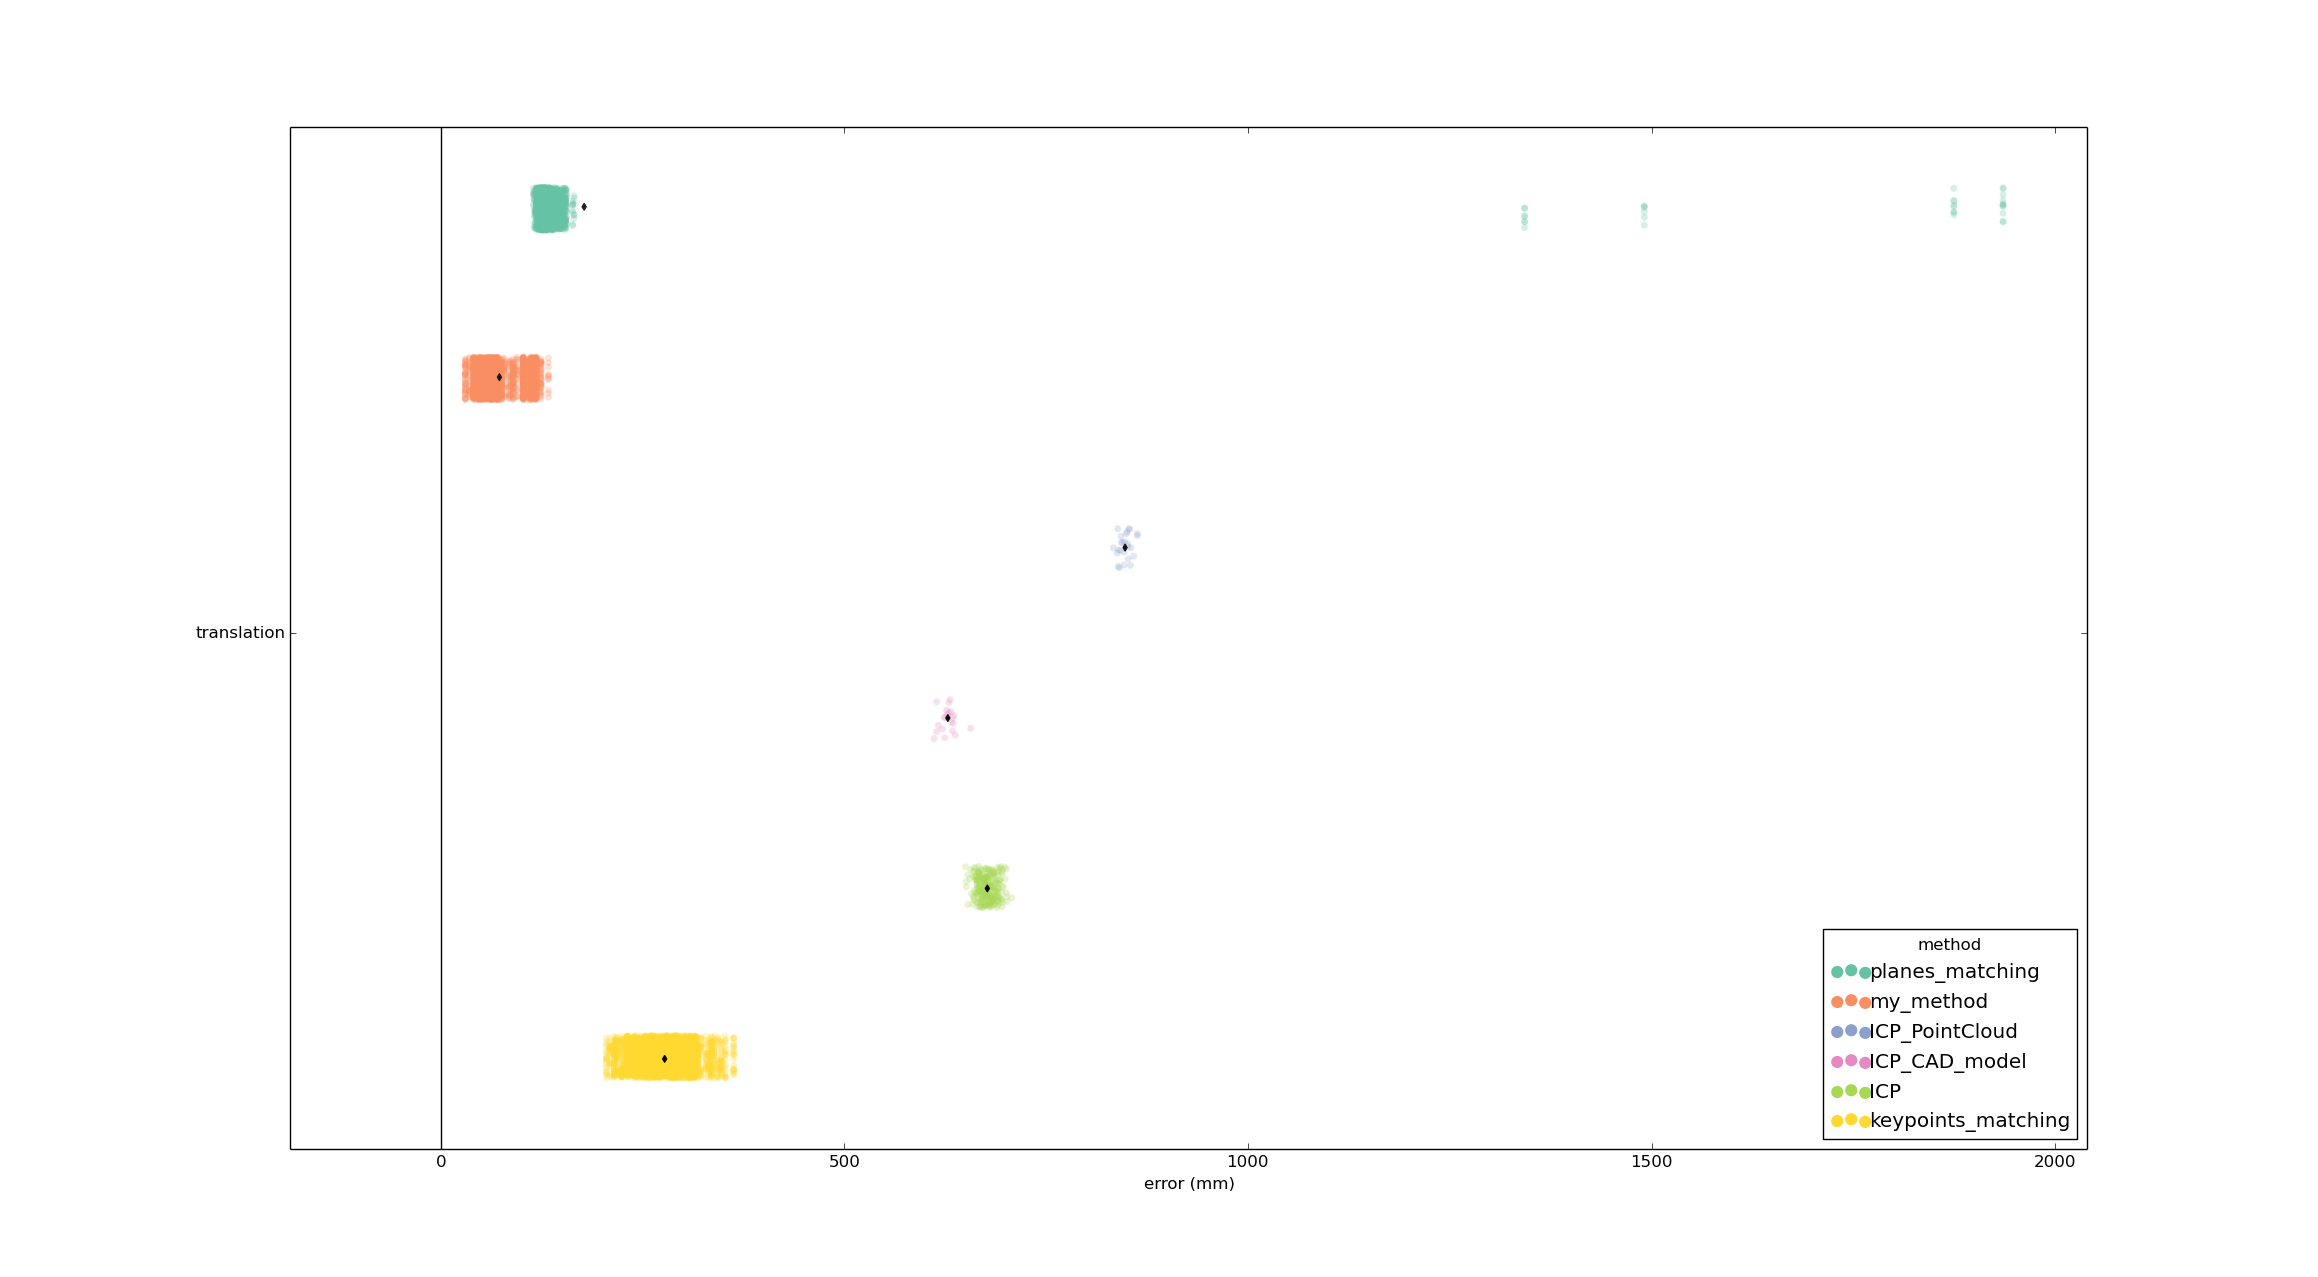
\includegraphics[width=\textwidth]{images/transl_comp.png}
    \caption{Comparison of overall translation error for each method.}
    \label{fig:trans_comp}
\end{figure}

\begin{figure}[h]
    \centering
    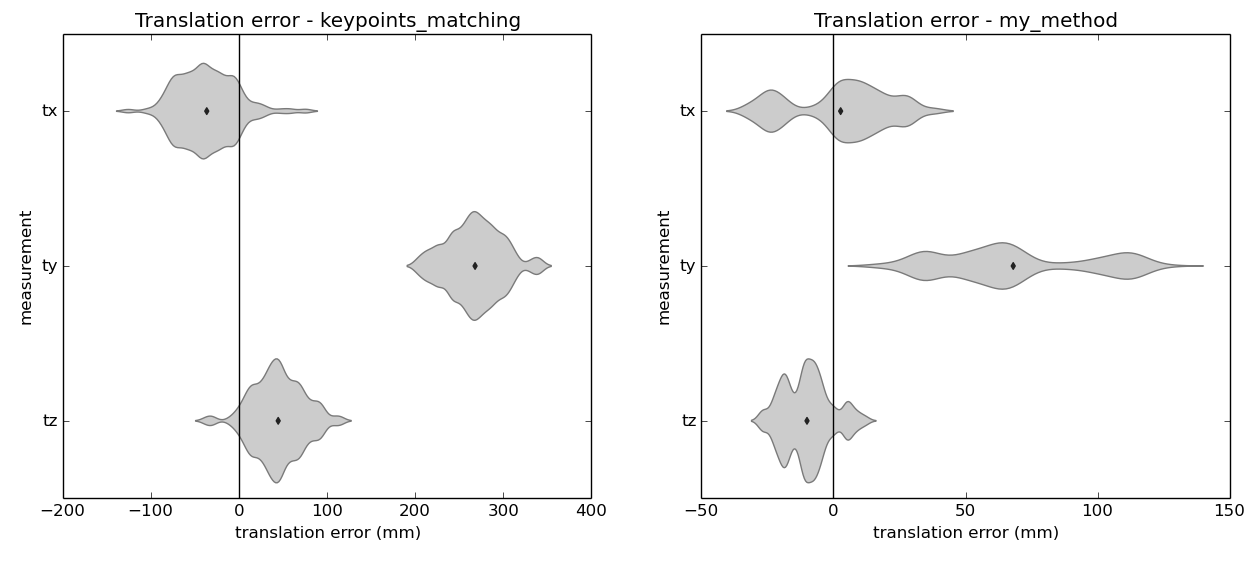
\includegraphics[width=\textwidth]{images/transl_violin.png}
    \caption{Detailed translation error distribution.}
    \label{fig:transl_violin}
\end{figure}

\begin{figure}[h]
    \centering
    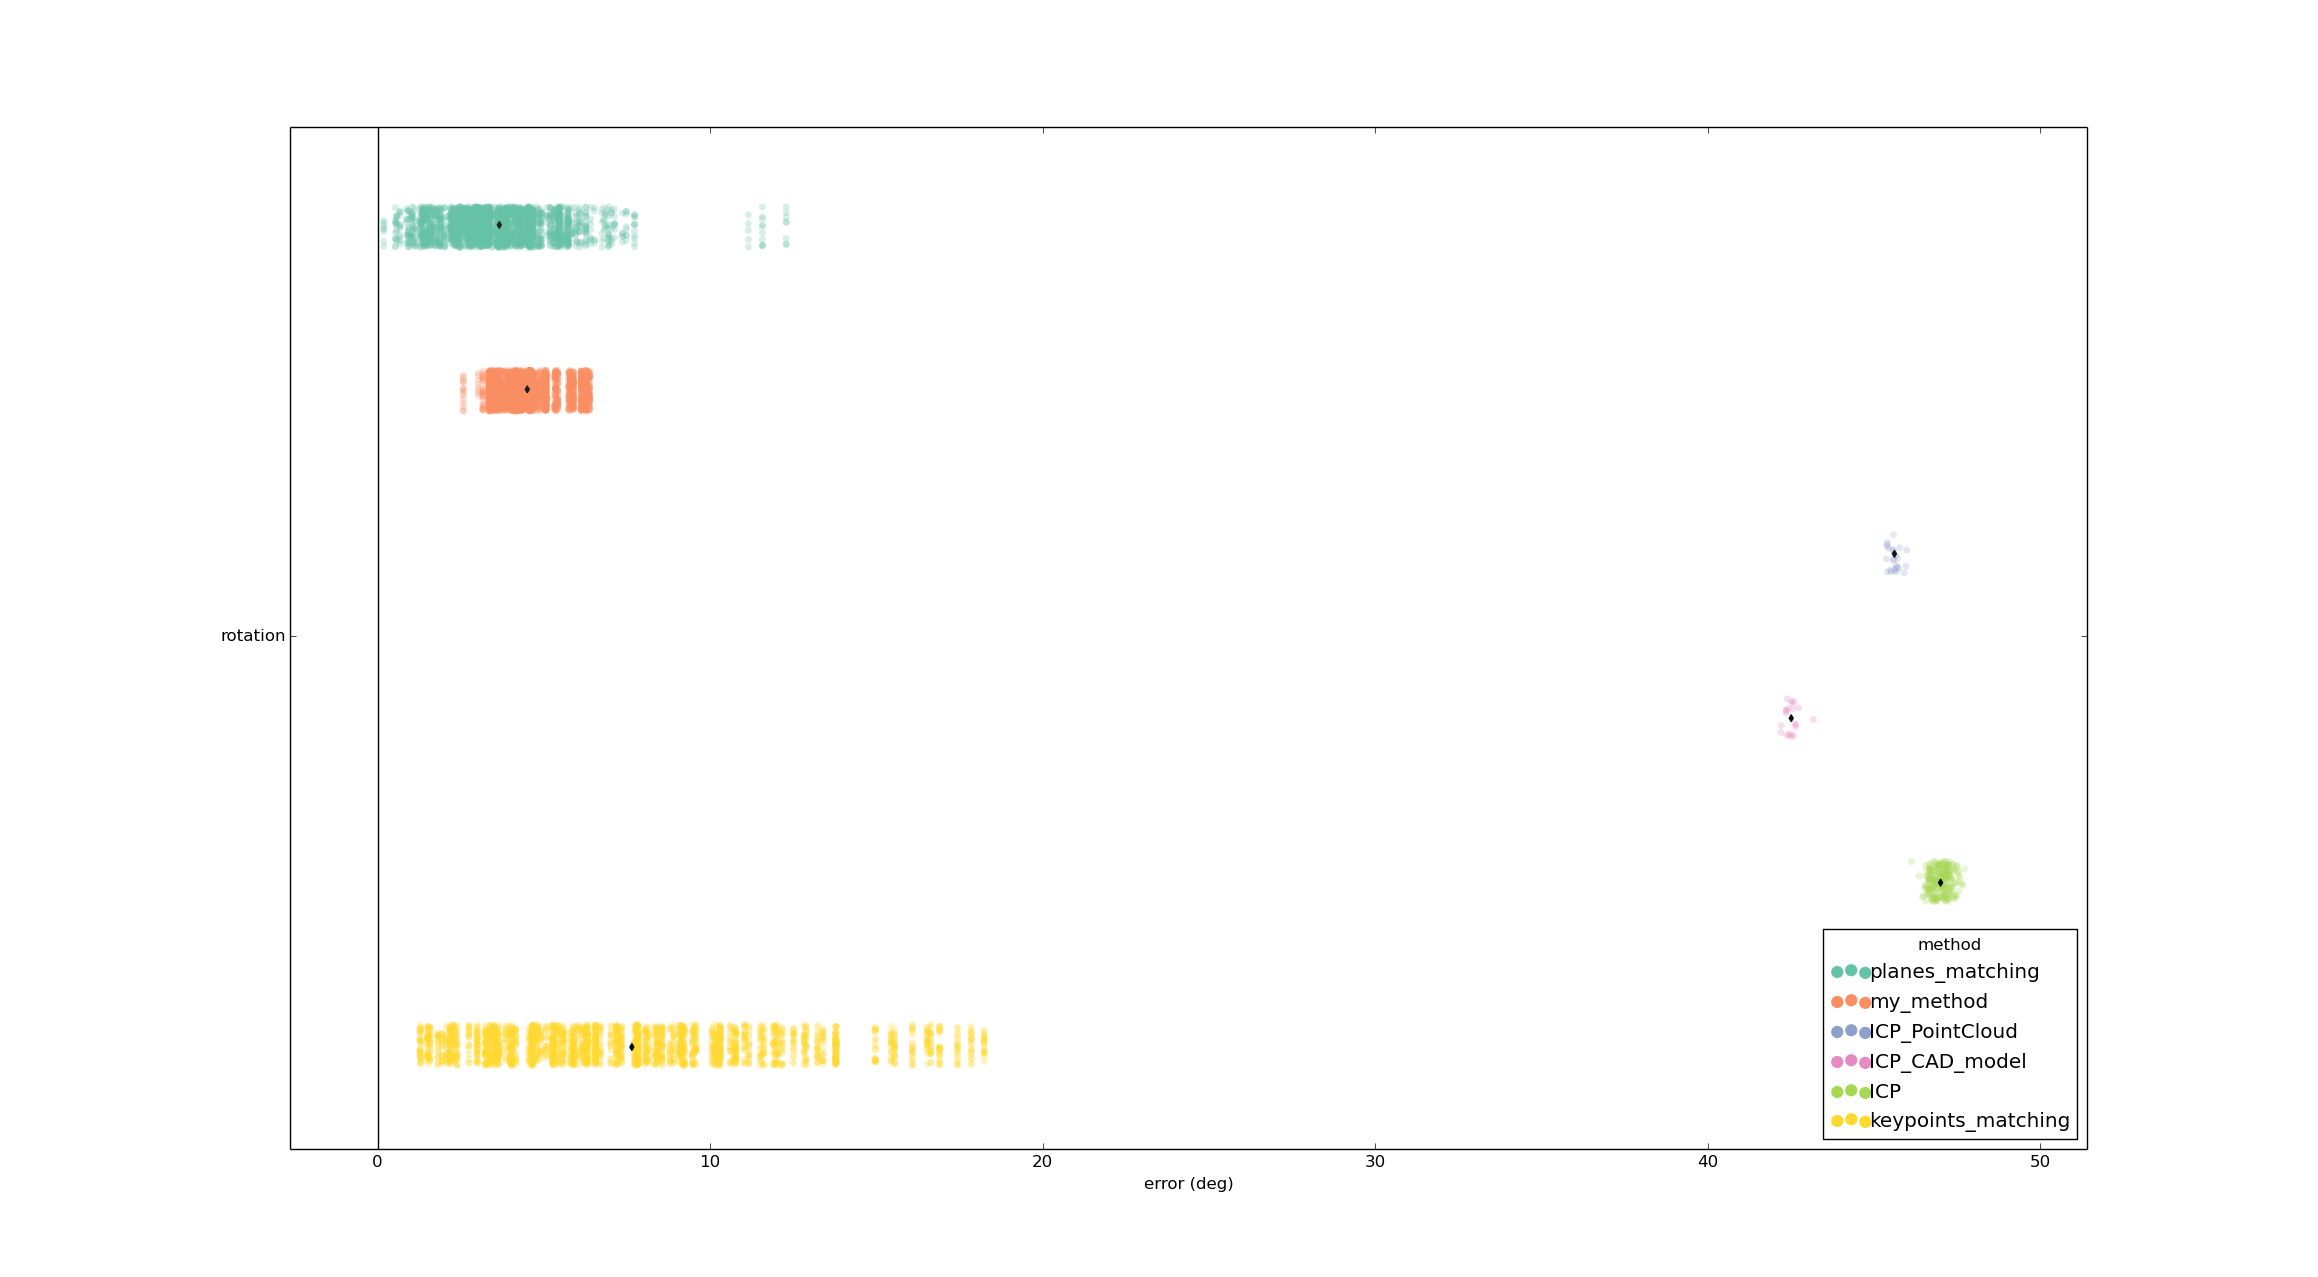
\includegraphics[width=\textwidth]{images/rot_comp.png}
    \caption{Comparison of overall rotation error for each method.}
    \label{fig:rot_comp}
\end{figure}

\begin{figure}[h]
    \centering
    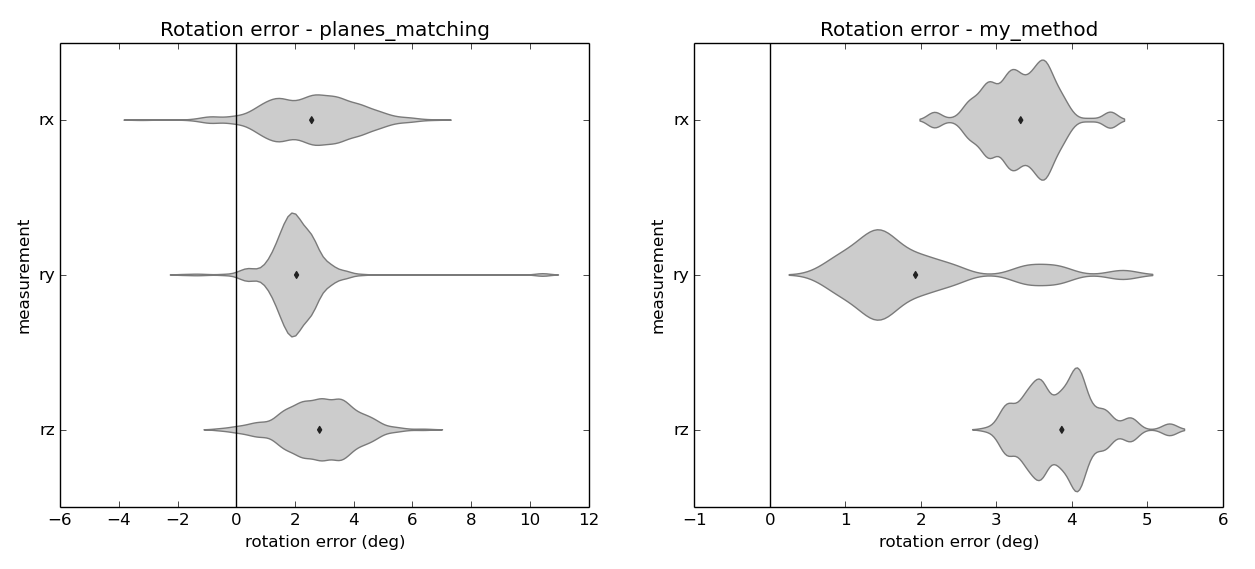
\includegraphics[width=\textwidth]{images/rot_violin.png}
    \caption{Detailed rotation error distribution.}
    \label{fig:rot_violin}
\end{figure}

We can notice that even for the mixed method, the standard deviation is larger for the Y translation estimation. This was expected due to the symmetry of the scene. This translation is determined only from keypoint matching and not from plane matching as other variables. Plane matching provides a precise translation estimation in the normal direction because it uses all the plane points position to align both clouds. Keypoints matching consists in matching few points that are determined with a large uncertainty.
However, as explained earlier, we can reduce the effect of these deviation by averaging the transform, especially during the first calibration process.

\subsection{Real Scenario with Small Initial Error}

In this experiment I start with an initial guess much smaller than in the previous one ; only $10^\circ$ of rotation on each axis and 20cm of translation. Even with this initial pose, the direct \acrshort{icp} method was not able to converge reliably to the solution, I was needed to tune really precisely the algorithm parameters for each attempt. I then choose to focus on matching methods since we are trying to compare automatic registration method and \acrshort{icp} registration can't be considered as an automatic method in this particular case.

\begin{figure}[h]
    \centering
    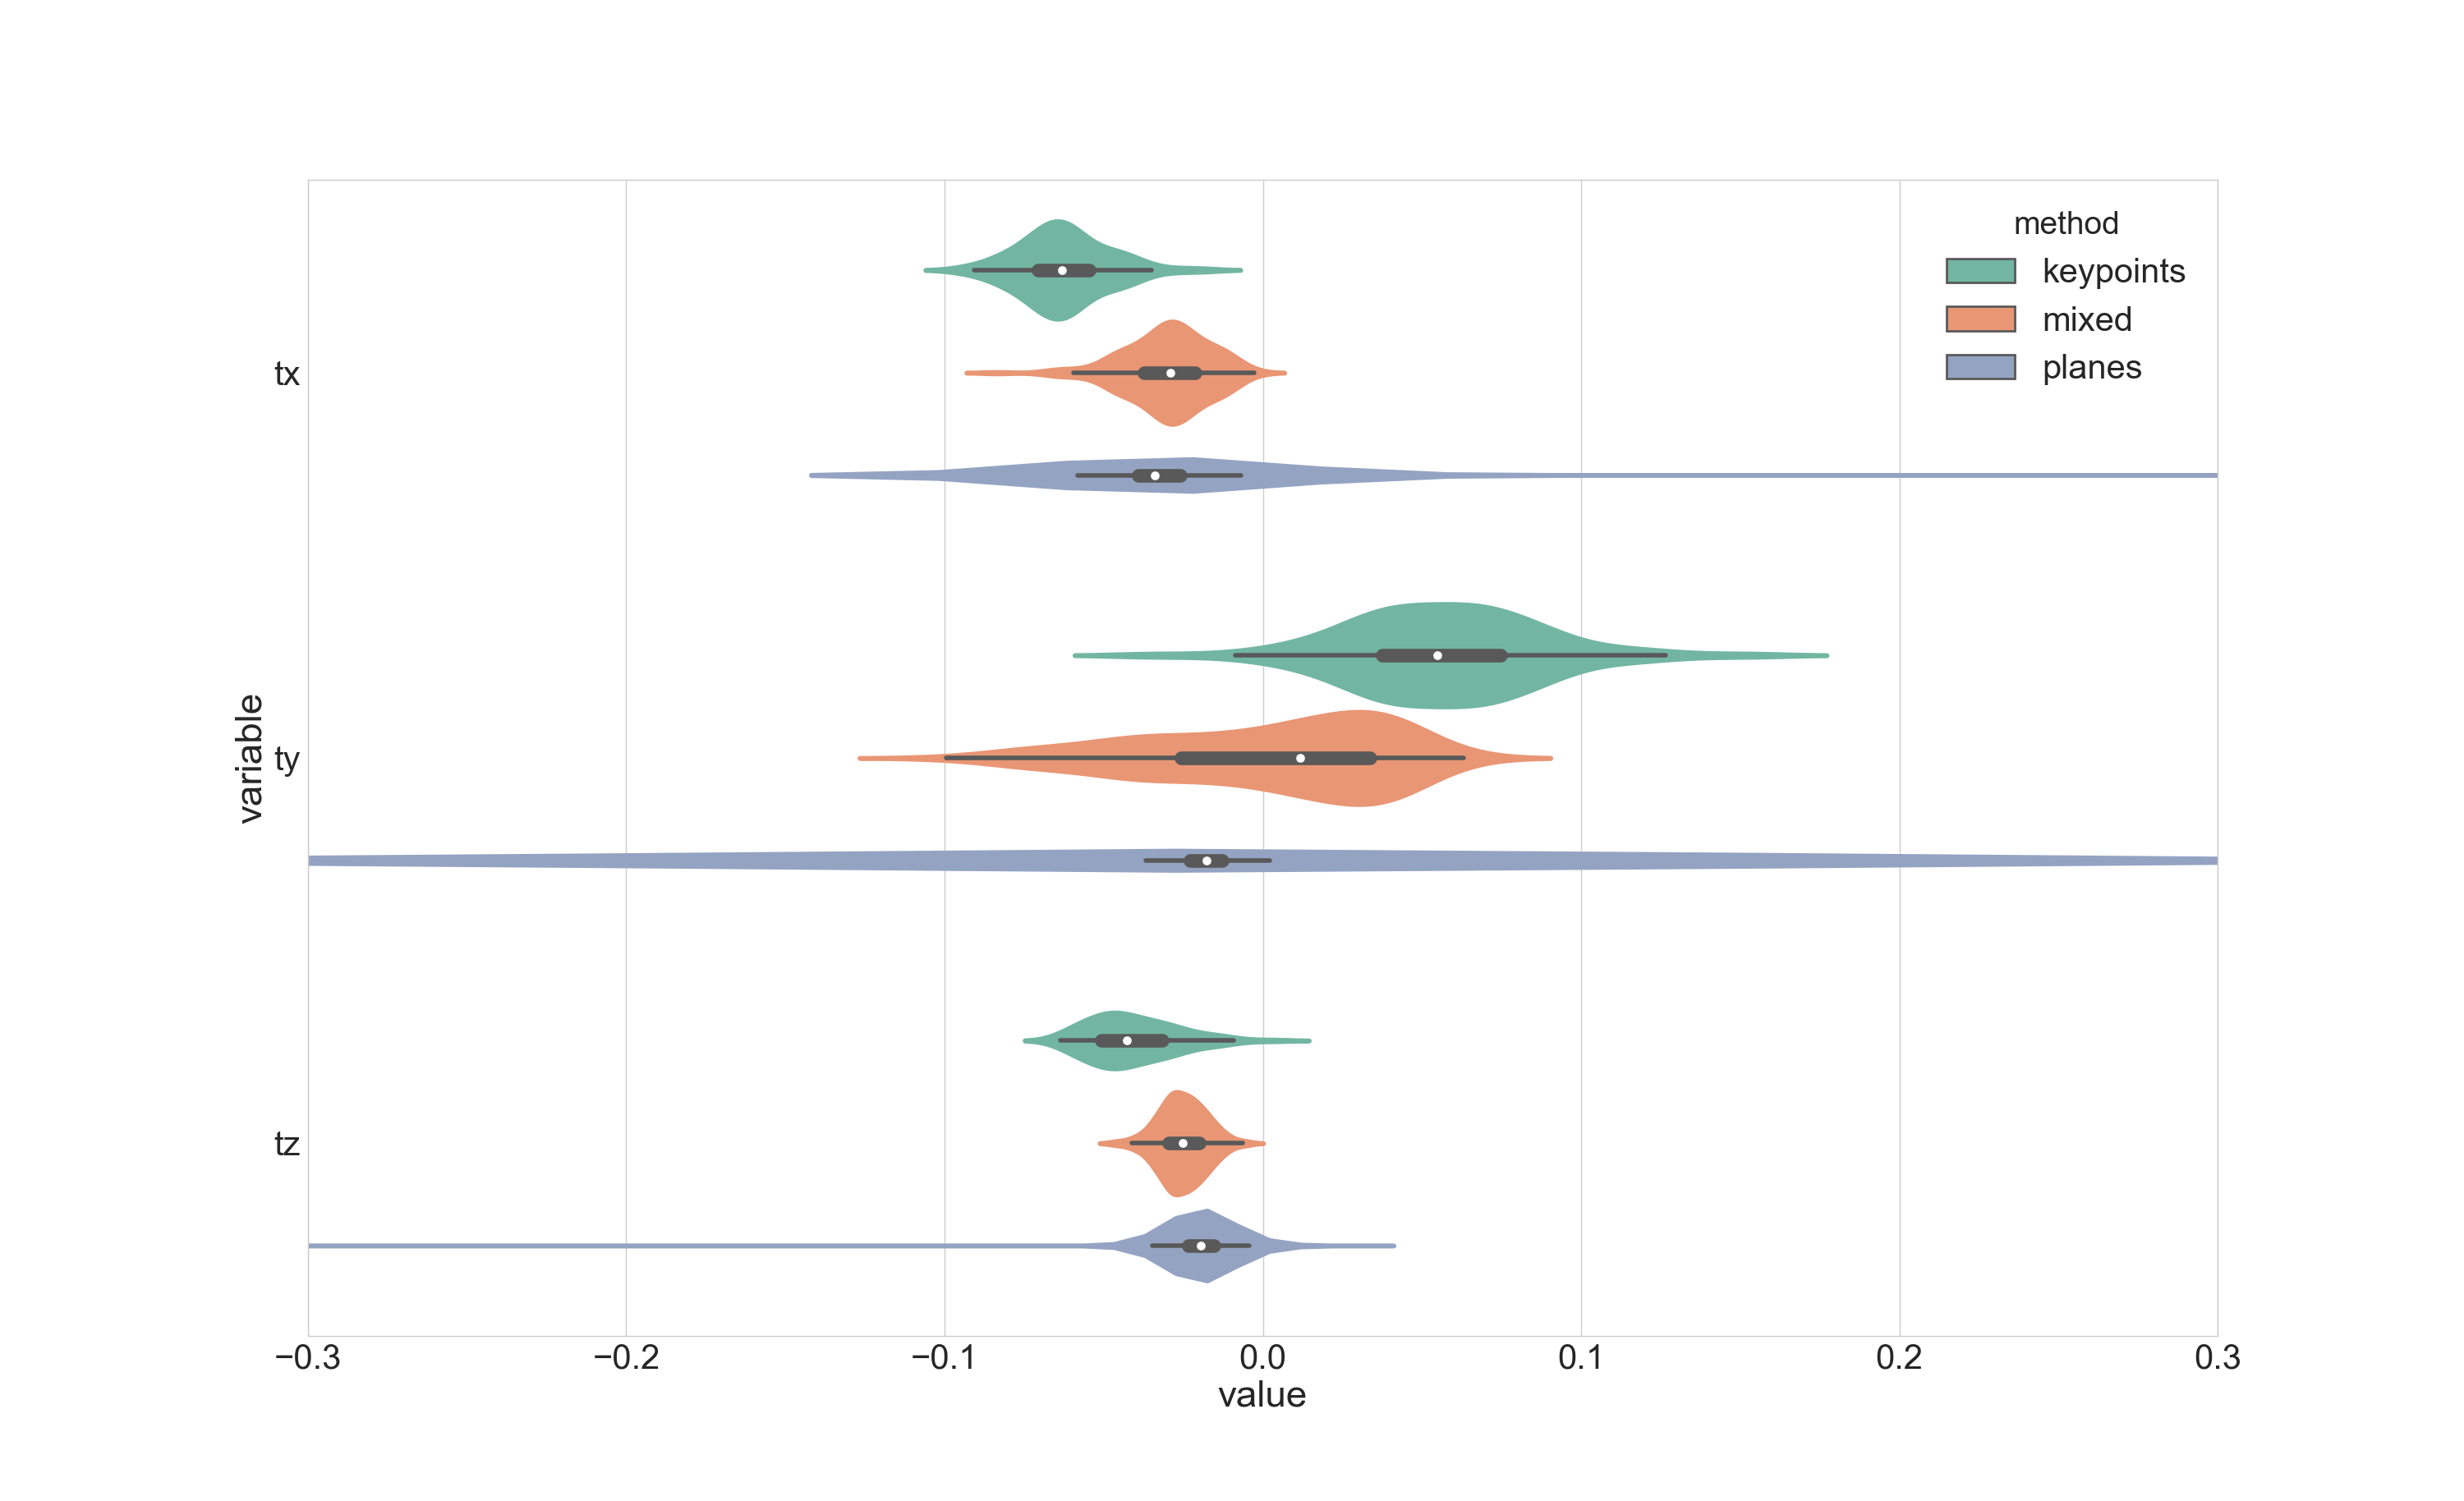
\includegraphics[width=\textwidth]{images/t_comp_small.png}
    \caption{Translation error distribution in m.\\White dot, thick and thin black lines correspond respectively to the median, interquartile range and 95\% confidence interval.}
    \label{fig:t_com}
\end{figure}

\begin{figure}[h]
    \centering
    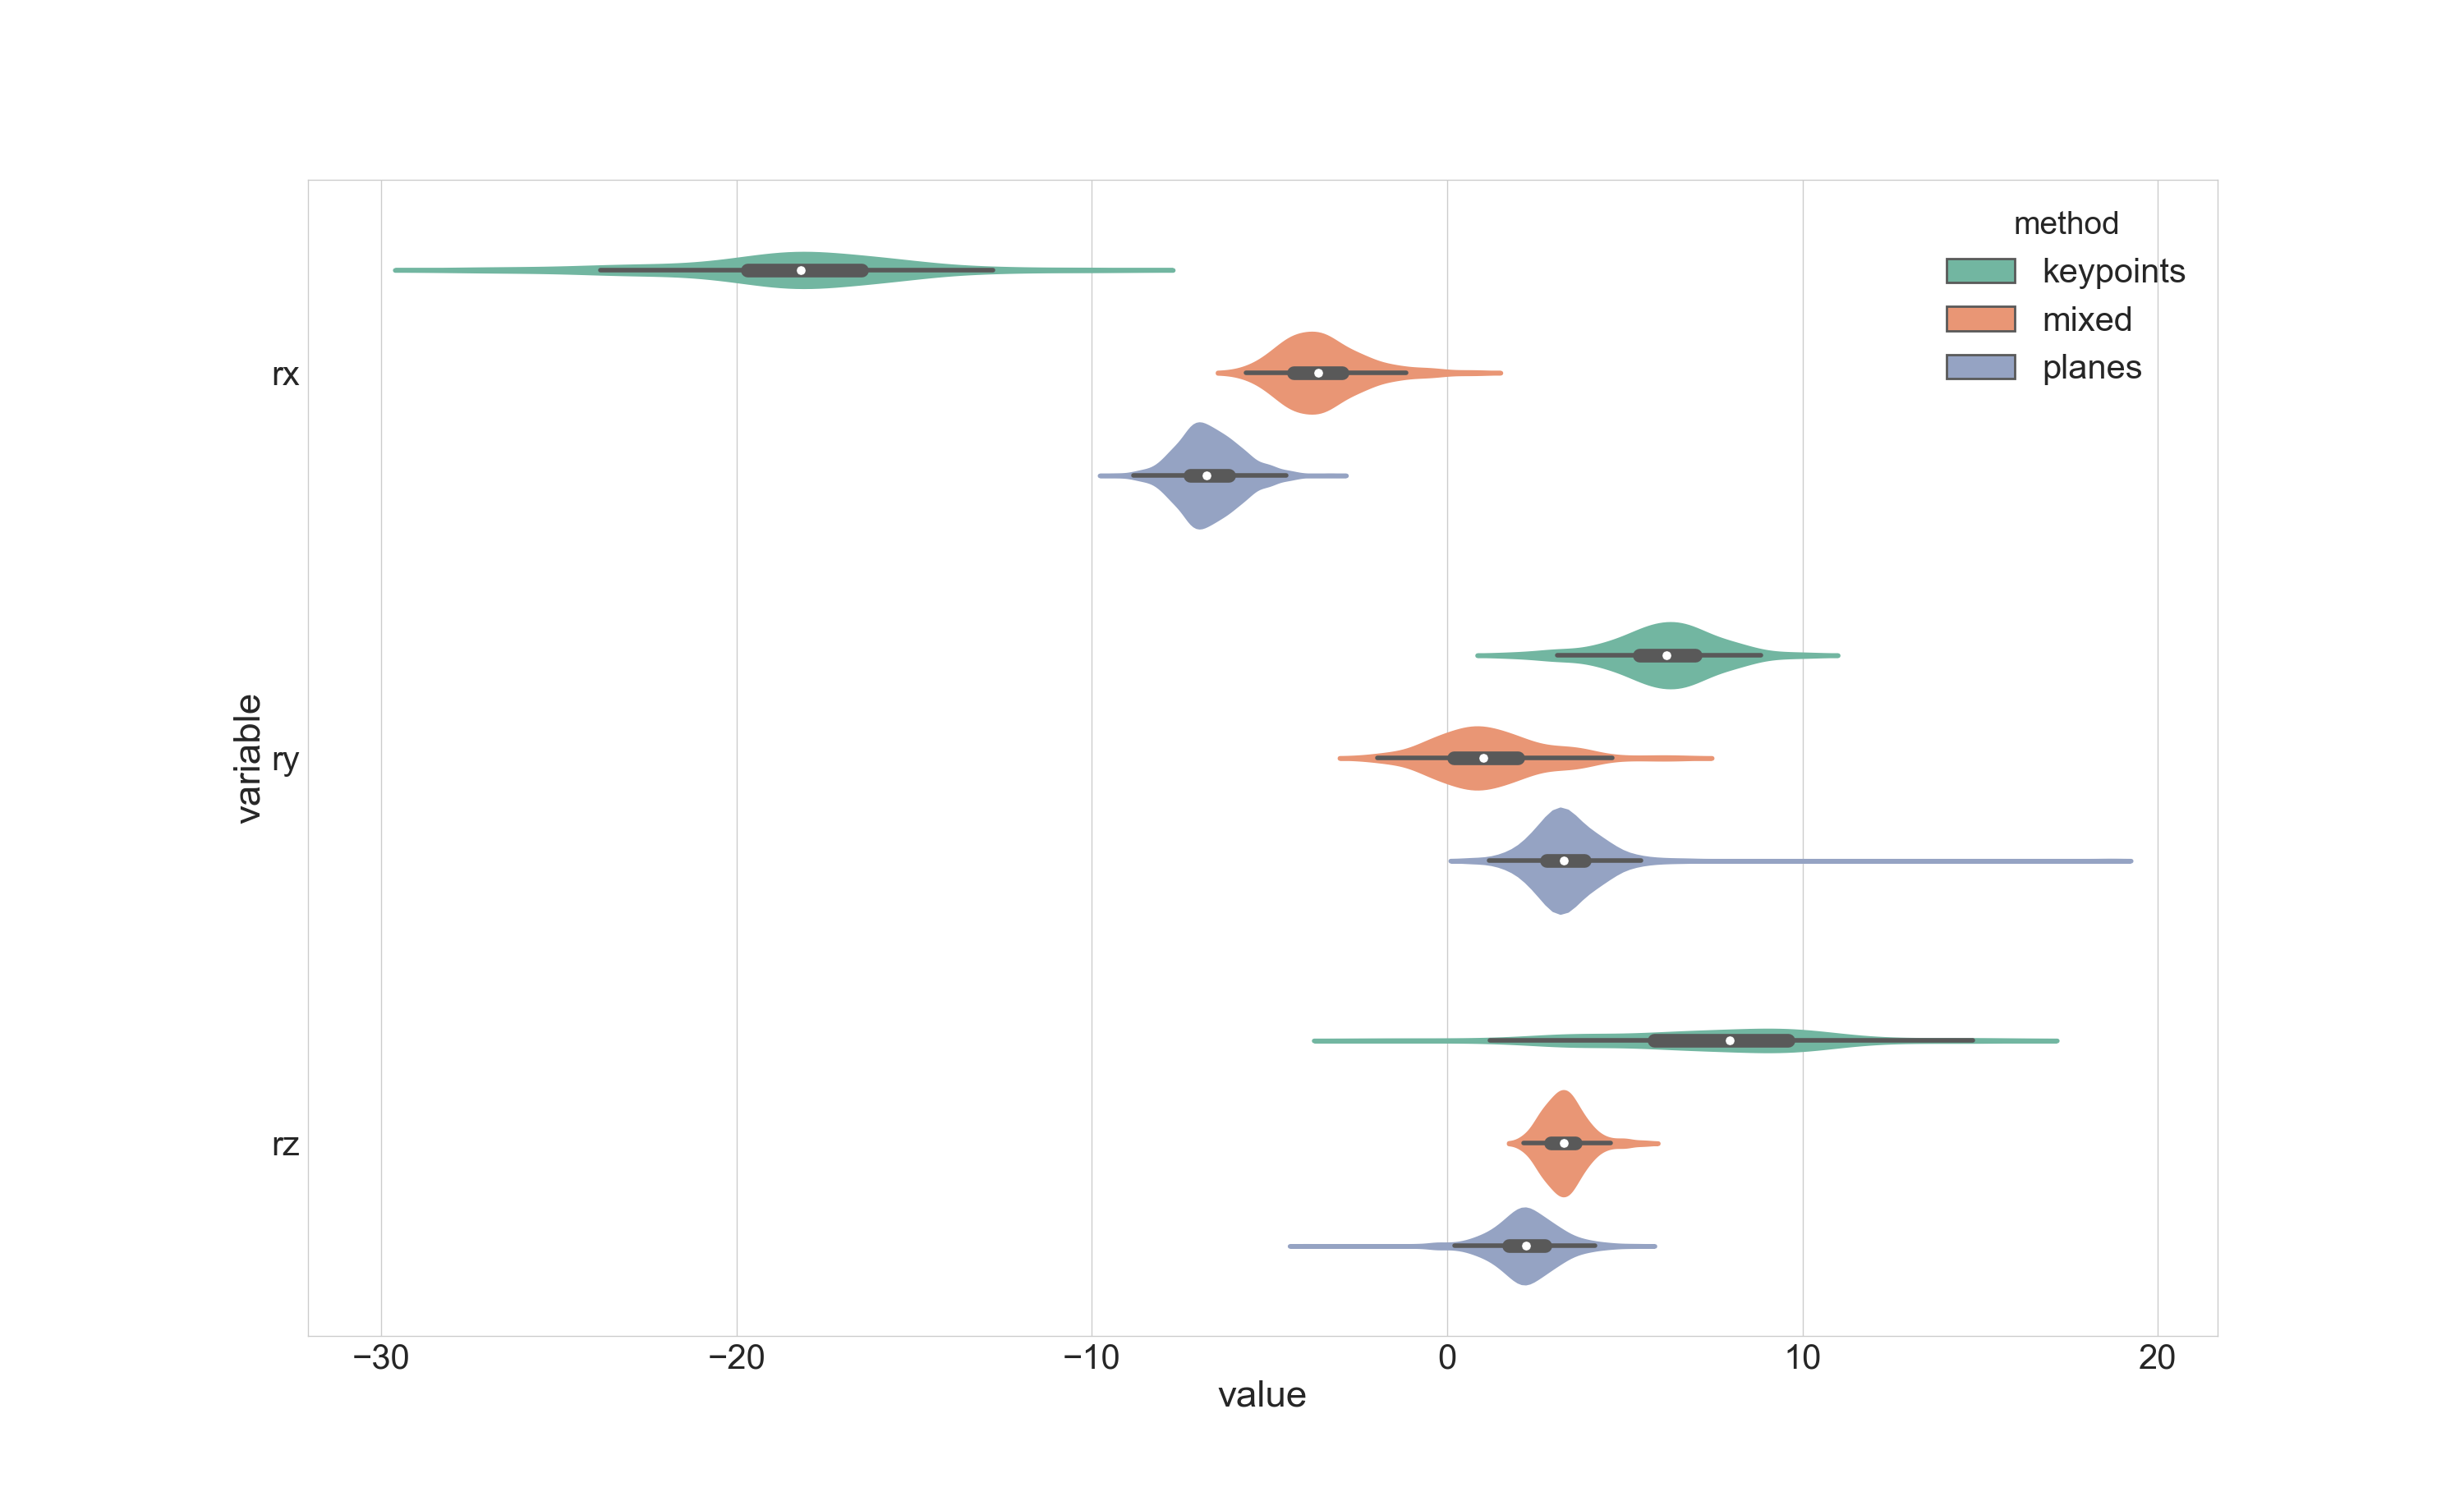
\includegraphics[width=\textwidth]{images/r_comp_small.png}
    \caption{Rotation error distribution in degrees.}
    \label{fig:r_comp}
\end{figure}

\begin{center}
    \begin{table}[h]
    \def\arraystretch{2}
    \centering
    \begin{tabular}{|c|c|c|c|}
    \hline
    Method                                                                        & Variable & Mean Value & Standard Deviation \\ \hline
    \multirow{6}{*}{\begin{tabular}[c]{@{}c@{}}Keypoints\\ Matching\end{tabular}} & tx       & -0.0625    & 0.0138             \\ \cline{2-4} 
              & ty       & 0.0569     & 0.0300             \\ \cline{2-4} 
              & tz       & -0.0409    & 0.0136             \\ \cline{2-4} 
              & rx       & -18.4      & 2.89               \\ \cline{2-4} 
              & ry       & 6.13       & 1.38               \\ \cline{2-4} 
              & rz       & 7.49       & 2.86               \\ \hline
    \multirow{6}{*}{\begin{tabular}[c]{@{}c@{}}Planes\\ Matching\end{tabular}}    & tx       & -0.0275    & 0.138              \\ \cline{2-4} 
              & ty       & -0.0410    & 0.620              \\ \cline{2-4} 
              & tz       & -0.0203    & 0.0331             \\ \cline{2-4} 
              & rx       & -6.69      & 0.842              \\ \cline{2-4} 
              & ry       & 3.36       & 1.04               \\ \cline{2-4} 
              & rz       & 2.22       & 0.891              \\ \hline
    \multirow{6}{*}{\begin{tabular}[c]{@{}c@{}}Mixed\\ Method\end{tabular}}      & tx       & -0.0300    & 0.0132             \\ \cline{2-4} 
              & ty       & 0.00243    & 0.0374             \\ \cline{2-4} 
              & tz       & -0.0252    & 0.00734            \\ \cline{2-4} 
              & rx       & -3.55      & 1.11               \\ \cline{2-4} 
              & ry       & 1.20       & 1.45               \\ \cline{2-4} 
              & rz       & 3.30       & 0.576              \\ \hline
    \end{tabular}
    \caption{Detailed mean and standard deviation for each variable. Translation in m and rotation in degrees.}
    \label{tabl:comp}
    \end{table}
\end{center}

In this experiment with a smaller initial error, our 3 matching methods behaviour is mostly unchanged. Mean values and standard deviation are detailed in table \ref{tabl:comp}.\\
First, we notice that planes matching method obtains values with a very large deviation in the translation estimation due to outlying values. These outliers can be caused by wrong plane matching or by an error in the plane detection. \\
For each method, the Y translation is also more spread out than the 2 other translations as we noticed in the first experiment. In the case of plane matching $ty$ uncertainty is very large because the $3^{rd}$ plane used to determine this translation is very deformed because it is placed in the overlapping region.\\
Keypoints matching method is, in contrary, less effective for rotation estimation, this can be understood as this method uses a matching of points only located in the center of the scene to align point clouds while methods using planes align planes that are defined by a large number of points spread out on the entire scene. Once again, the rotation estimation is slightly better with the mixed method than the plane matching.

\section{Computing Speed}

We can evaluate algorithm's speed by comparing the number of transform estimation provided during the experiment and compute the number of frames (or estimations) per second. \\
The fastest algorithm is by far plane matching registration because it only involves \acrshort{ransac} planes detection which doesn't need a lot of computation. In contrary the keypoint detection, feature estimation and matching used in other methods is needing a lot more computation. The reason why the mixed methods is faster than keypoints matching only is that as it is based mainly on plane detection, only few keypoints are needed and only objects in the overlapping region are considered while keypoints matching needs to detect keypoints also on the table and wall to be accurate which leads to the need of processing a lot more keypoints.

\begin{table}[h]
    \def\arraystretch{2}
    \centering
    \begin{tabular}{|c|c|}
    \hline
    Method          & FPS  \\ \hline
    Keypoints       & 0.84 \\ \hline
    Planes          & 7.58 \\ \hline
    Mixed           & 1.59 \\ \hline
    \end{tabular}
    \caption{Computing speed during the first experiment (in \acrshort{fps}).}
    \label{tabl:speed}
\end{table}

